\section{Auswertung}
\subsection{Ablenkung im elektrischen Feld}
Es werden die Messdaten der Strahlablenkung $D$, der Plattenspannung $U_d$ und die Beschleunigungsspannung $U_B$ notiert.
Sie sind in der Tabelle \ref{tab:1} dargestellt.
\begin{table}[H]
  \centering
  \caption{Messdatendarstellung.}
  \label{tab:1}
  \begin{tabular}{c c c c c c}
\toprule
& \multicolumn{1}{c}{$U_B=\SI{200}{\volt}$} & \multicolumn{1}{c}{$U_B=\SI{250}{\volt}$} &\multicolumn{1}{c}{$U_B=\SI{300}{\volt}$}&\multicolumn{1}{c}{$U_B=\SI{400}{\volt}$}&\multicolumn{1}{c}{$U_B=\SI{500}{\volt}$}\\
\cmidrule(lr){2-2}\cmidrule(lr){3-3}\cmidrule(lr){4-4}\cmidrule(lr){5-5}\cmidrule(lr){6-6}
$D \, / \, \si{\centi\meter}$ & $U_d \, / \, \si{\volt}$ & $U_d \, / \, \si{\volt}$ & $U_d \, / \, \si{\volt}$ &$U_d \, / \, \si{\volt}$ & $U_d \, / \, \si{\volt}$\\
\midrule
5.080 & 21,9  & 28,9  & 33,8  & -    & -   \\
4.445 & 19,1  & 24,6  & 29,0  & -    & -   \\
3.810 & 14,9  & 19,6  & 23,3  & 30,7 & -   \\
3.175 & 11,2  & 14,6  & 17,2  & 22,9 & 31,3\\
2.540 &  6,5  &  8,5  & 10,2  & 14,7 & 21,2\\
1.905 &  2,5  &  4,5  &  4,7  &  6,1 & 10,2\\
1.270 & -1,6  & -0,7  & -1,6  & -1,0 & -0,5\\
0.635 & -5,3  & -5,9  & -7,4  & -9,2 &-11,3\\
0.000 & -9,3  &-10,6  &-13,9  &-17,0 &-21,6\\
\bottomrule
  \end{tabular}
\end{table}
Für jede einzelne Beschleunigungsspannung $U_b$ werden die
Parameter $D$ und $U_d$ gegeneinander aufgetragen.
Die jeweils linearen Ausgleichsrechnungen wurde mit Python 3.6 durchgeführt.
Für den Fit wird Gleichung \ref{eq:1} verwendet:
\begin{equation*}
  \underbrace{D}_{\mathclap{y}} = \underbrace{\frac{pL}{2dU_B}}_{\mathclap{m}} \cdot \underbrace{U_d}_{\mathclap{x}} + \, b
\end{equation*}
Dabei ist $b$ der Y-Achsenschnitt.

In der Abbildung \ref{abb:6} ist die Darstellung von der Beschleunigungsspannung $U_b=\SI{200}{\volt}$.
\begin{figure}[H]
  \centering
  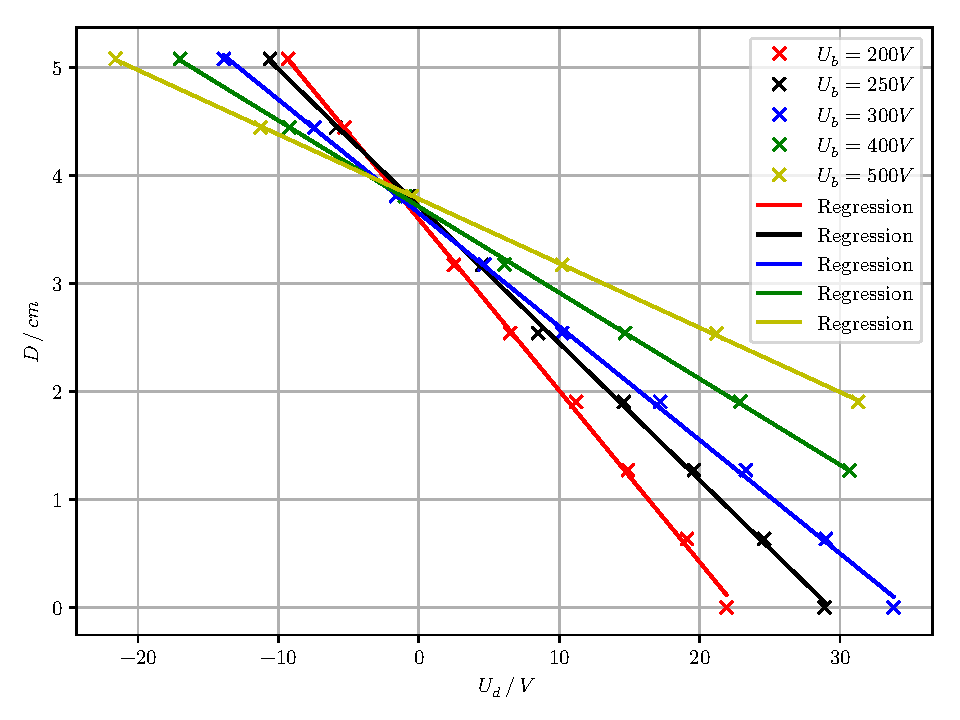
\includegraphics{plot1.pdf}
  \caption{Darstellung von $U_b= \SI{200}{\volt}$.}
  \label{abb:6}
\end{figure}
Es ergibt sich hierfür die Parameter
\begin{itemize}
  \item $m=\SI{0.1587(22)}{\centi\meter\per\volt}$
  \item $b=\SI{1.4835(0265)}{\centi\meter}$
\end{itemize}
In der nächsten Abbildung \ref{abb:7} ist die Darstellung von der Beschleunigungsspannung $U_b=\SI{250}{\volt}$.
\begin{figure}[H]
  \centering
  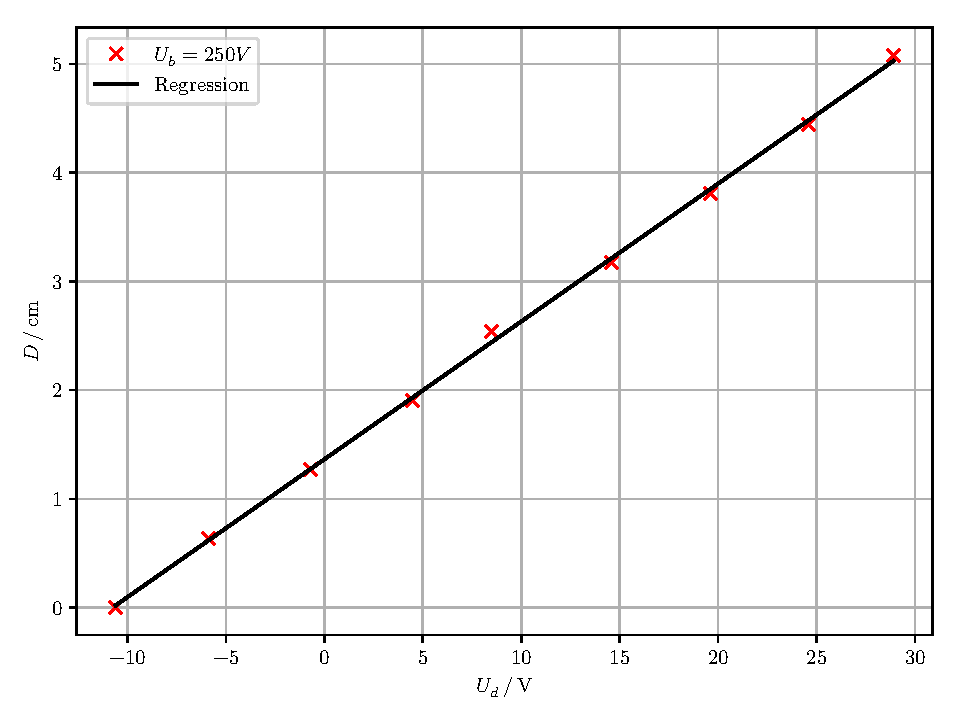
\includegraphics{plot2.pdf}
  \caption{Darstellung von $U_b=\SI{250}{\volt}$.}
  \label{abb:7}
\end{figure}
Es ergibt sich hierfür die Parameter
\begin{itemize}
  \item $m=\SI{0.1268(13)}{\centi\meter\per\volt}$
  \item $b=\SI{1.3634(0211)}{\centi\meter}$
\end{itemize}
In der nächsten Abbildung \ref{abb:8} ist die Darstellung von der Beschleunigungsspannung $U_b=\SI{300}{\volt}$.
\begin{figure}[H]
  \centering
  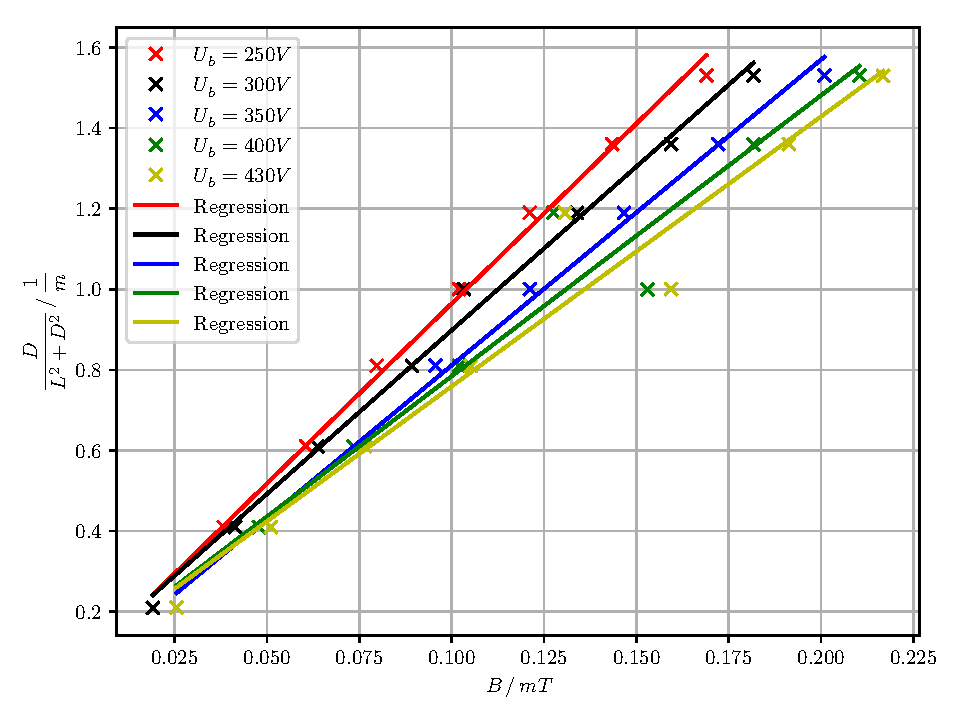
\includegraphics{plot3.pdf}
  \caption{Darstellung von $U_b=\SI{300}{\volt}$.}
  \label{abb:8}
\end{figure}
Es ergibt sich hierfür die Parameter
\begin{itemize}
  \item $m=\SI{0.1051(12)}{\centi\meter\per\volt}$
  \item $b=\SI{1.4275(0228)}{\centi\meter}$
\end{itemize}
In der nächsten Abbildung \ref{abb:9} ist die Darstellung von der Beschleunigungsspannung $U_b=\SI{400}{\volt}$.
\begin{figure}[H]
  \centering
  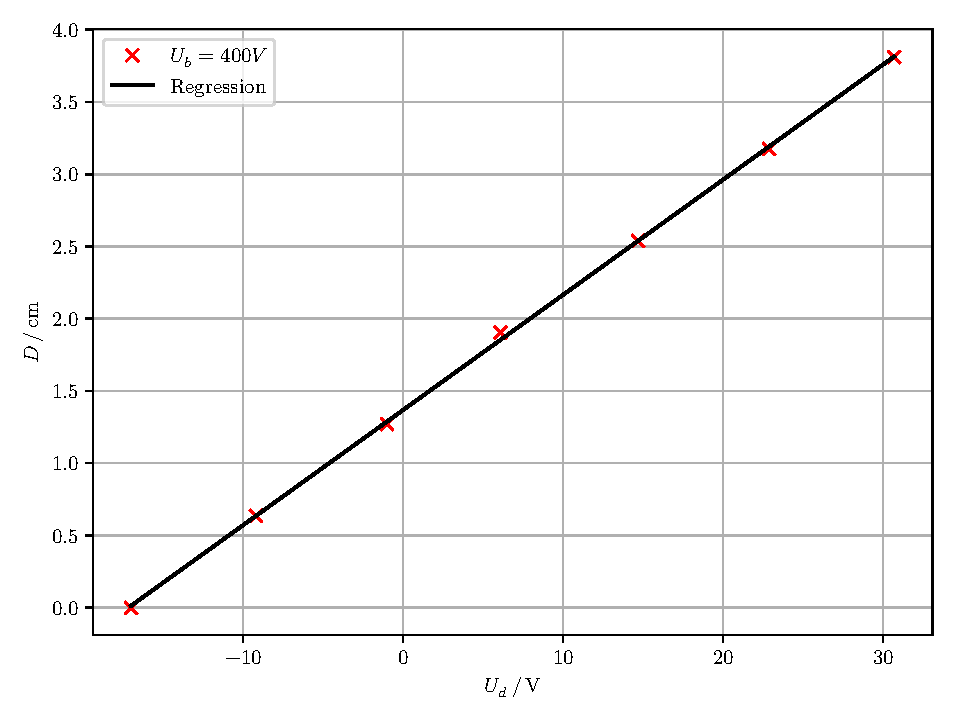
\includegraphics{plot4.pdf}
  \caption{Darstellung von $U_b=\SI{300}{\volt}$.}
  \label{abb:9}
\end{figure}
Es ergibt sich hierfür die Parameter
\begin{itemize}
  \item $m=\SI{0.0797(6)}{\centi\meter\per\volt}$
  \item $b=\SI{1.3675(0108)}{\centi\meter}$
\end{itemize}
In der nächsten Abbildung \ref{abb:10} ist die Darstellung von der Beschleunigungsspannung $U_b=\SI{500}{\volt}$.
\begin{figure}[H]
  \centering
  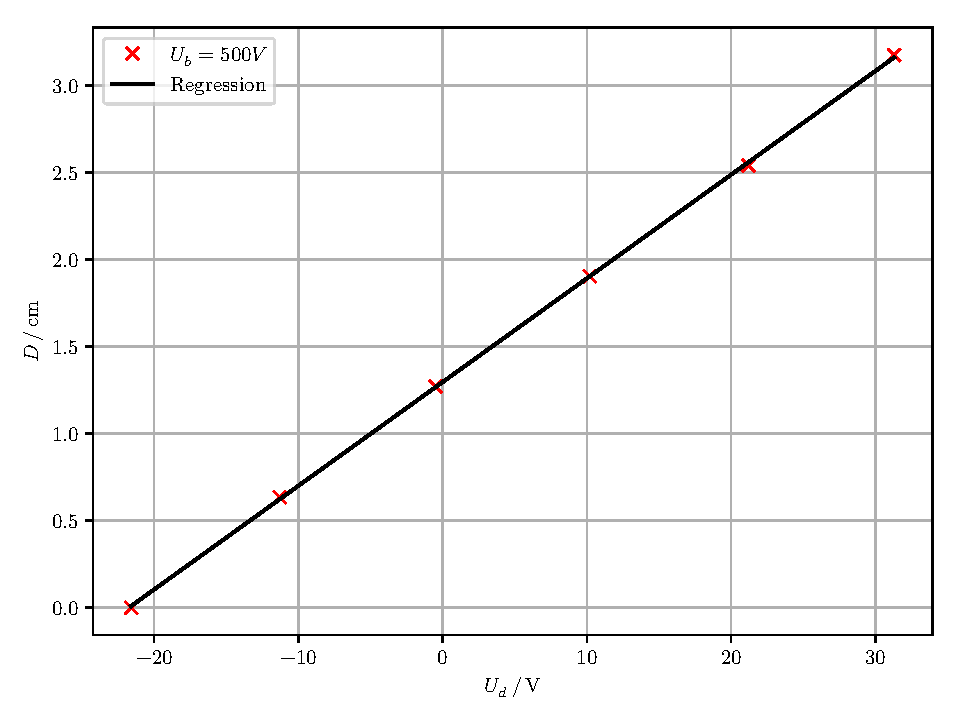
\includegraphics{plot5.pdf}
  \caption{Darstellung von $U_b=\SI{500}{\volt}$.}
  \label{abb:10}
\end{figure}
Es ergibt sich hierfür die Parameter
\begin{itemize}
  \item $m=\SI{0.0596(3)}{\centi\meter\per\volt}$
  \item $b=\SI{1.2963(0060)}{\centi\meter}$
\end{itemize}
Relevant für die Bestimmung der Konstruktionskonstante $a$ sind die jeweiligen Steigungen $m_i \,\text{für} \, i \in [1,2,3,4,5]$.
Sie werden in der folgenden Tabelle \ref{tab:2} erneut dargestellt.
\begin{table}[H]
  \centering
  \caption{Ergebnis der jeweiligen Steigungen $m_i$.}
  \label{tab:2}
  \begin{tabular}{c c c}
\toprule
&$\text{Steigung} \,/\, \si{\centi\meter\per\volt}$& $U_B \, /\, \si{\volt}$\\
\midrule
$m_1$ & $\num{0.1587(22)}$& 200\\
$m_2$ & $\num{0.1268(13)}$& 250\\
$m_3$ & $\num{0.1051(12)}$& 300\\
$m_4$ & $\num{0.0797(6)}$ & 400\\
$m_5$ & $\num{0.0596(3)}$ & 500\\
\bottomrule
  \end{tabular}
\end{table}
Die bestimmten Steigungen sind die Empfindlichkeiten $\frac{D}{U_d}$ der Kathodenstrahlröhre.
Diese werden nun gegen $\frac{1}{U_B}$ aufgetragen.
Die Darstellung ist in Abbildung \ref{abb:11} zu sehen.
\begin{figure}[H]
  \centering
  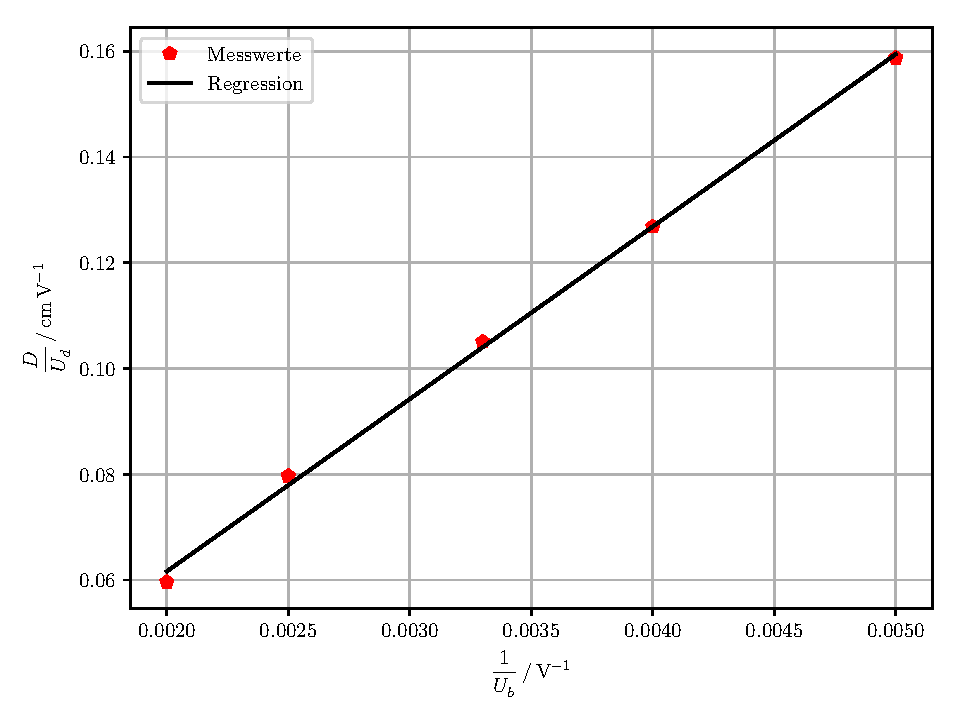
\includegraphics[width=\textwidth]{plot6.pdf}
  \caption{Darstellung zur Bestimmung der Konstruktionskonstanten $a$.}
  \label{abb:11}
\end{figure}
Auch hier wurde eine lineare Ausgleichsrechnung mit Python 3.6 durchgeführt.
Dazu wurde die Gleichung \ref{eq:1} erneut verwendet:
\begin{equation*}
  \underbrace{\frac{D}{U_d}}_{\mathclap{y}} = \underbrace{\frac{pL}{2d}}_{\mathclap{a}} \cdot \underbrace{\frac{1}{U_B}}_{\mathclap{x}} + b
\end{equation*}
Es folgt somit für die Konstruktionskonstante $a$
\begin{equation*}
  a = \SI{32,59(72)}{\centi\meter}.
\end{equation*}
Für den Y-Achsenschnitt $b$
\begin{equation*}
  b = \SI{-0.00354(00252)}{\centi\meter\per\volt}
\end{equation*}

Der theoretische Wert kann mithilfe der Abbildung \ref{abb:5} bestimmt werden.
Dabei ist
\begin{itemize}
  \item $p = \SI{1.9}{\centi\meter}$
  \item $L = \SI{15.33}{\centi\meter}$
  \item $d = \SI{0.665}{\centi\meter}$
\end{itemize}
Der $L$-Wert ergibt sich aus zwei Komponenten. Einmal der Abstand Kondensatorplatte bis
zum Leuchtschirm, welcher $\SI{14.3}{\centi\meter}$ beträgt und zum anderen noch die Länge
der Kondensatorplatten, die $\SI{1.03}{\centi\meter}$ ist.
Der $d$-Wert ist der Mittelwert von den beiden Plattenabständen der Kondensatorplatten.
Es folgt somit für die Konstruktionskonstante
\begin{equation*}
  a_{\text{Theo}} = \frac{pL}{2d} = \SI{21.9}{\centi\meter}
\end{equation*}

Es wird nun die Frequenz der Sinusspannung mithilfe der Sägezahnspannung
berechnet.
Dazu wird die Gleichung \ref{eq:2} genutzt. Dabei ist $m = 1$ und der
Proportionalitätsfaktor $n= 0.5, 1, 2, 3$
Die Messwerte werden in die Gleichung \ref{eq:2} eingesetzt und somit wird die Sinusfrequenz berechnet.
Die Ergebnisse sind in der Tabelle \ref{tab:3} dargestellt.
\begin{table}[H]
  \centering
  \caption{Ergebnisse zur Bestimmung der Sinusspannung.}
  \label{tab:3}
  \begin{tabular}{c c c}
\toprule
$\nu_{Sä} \,/\, \si{\hertz}$& $\text{Proportionalitätsfaktor}$ & $\nu_{Si} \, /\, \si{\hertz}$\\
\midrule
29,33 & 3 & 87,99\\
49,99 & 2 & 99,98\\
79,32 & 1 & 79,32\\
158,64& 0,5& 79,32\\
\bottomrule
  \end{tabular}
\end{table}
Die Ergebnisse werden nun gemittelt.
Für den Mittelwert sowie Standardabweichung des Mittelwerts werden die folgenden Gleichungen verwendet:
\begin{equation*}
    \bar{\nu}_{Si}= \frac{1}{N} \sum_{i=1}^{N} \nu_{Si,i}
\end{equation*}

\begin{equation*}
  \Delta \bar{\nu}_{Si} = \frac{1}{\sqrt{N}\sqrt{N-1}} \sqrt{\sum_{i}(\nu_{Si,i}-\bar{\nu}_{si})^2}
\end{equation*}
verwendet.
Es folgt für die Frequenz der Sinusspannung:
\begin{equation*}
  \nu_{si}= \SI{86.65(488)}{\hertz}
\end{equation*}
Des Weiteren soll der Scheitelwert mithilfe der Strahlablenkung $D$ und der Konstruktionskonstante $a$ berechnet werden.
Es wurde eine Beschleunigungsspannung $U_b = \SI{300}{\volt}$ angelegt. Die gemessene Konstruktionskonstante ist
$a = \SI{32,59(72)}{\centi\meter}$.
Bei den Messungen ergab sich eine konstante Strahlablenkung von $D = \SI{1.905}{\centi\meter}$.
Nun kann die Gleichung \ref{eq:1} umgeformt werden nach  der Plattenspannung $U_d$.
Es folgt:
\begin{equation*}
  U_d = \frac{D U_B}{a} = \SI{17.5(4)}{\volt}
\end{equation*}
Der Fehler lässt sich mithilfe der Gauß´schen Fehlerfortpflanzung wie gefolgt bestimmen
\begin{equation}
  \Delta U_d = \sqrt{\Bigl(-\frac{DU_B}{a^2}\cdot \Delta a\Bigr)^2}
\end{equation}
\subsection{Ablenkung im magnetischen Feld}
Um die spezifische Ladung der Elektronen bestimmen zu können, werden zunächst
die Messwerte der Ablenkung $D$, des Stromes $I$, der durch die Helmholzspule geht, sowie der
Beschleunigungsspannung $U_B$ notiert.
Die Ergebnisse sind in der Tabelle \ref{tab:4} dargestellt.
\begin{table}[H]
  \centering
  \caption{Ergebnisse der Messdatenaufzeichnungen.}
  \label{tab:4}
  \begin{tabular}{c c c c c c}
\toprule
& \multicolumn{1}{c}{$U_B=\SI{200}{\volt}$} & \multicolumn{1}{c}{$U_B=\SI{250}{\volt}$} &\multicolumn{1}{c}{$U_B=\SI{300}{\volt}$}&\multicolumn{1}{c}{$U_B=\SI{400}{\volt}$}&\multicolumn{1}{c}{$U_B=\SI{500}{\volt}$}\\
\cmidrule(lr){2-2}\cmidrule(lr){3-3}\cmidrule(lr){4-4}\cmidrule(lr){5-5}\cmidrule(lr){6-6}
$D \, / \, \si{\centi\meter}$ & $I \, / \, \si{\ampere}$ & $I \, / \, \si{\ampere}$ & $I \, / \, \si{\ampere}$ &$I \, / \, \si{\ampere}$ & $I \, / \, \si{\ampere}$\\
\midrule
0,635 & 0,30  & 0,30 & 0,40 & 0,40& 0,40\\
1,270 & 0,60  & 0,65 & 0,75 & 0,75& 0,80\\
1,905 & 0.95  & 1,00 & 1,15 & 1,15& 1,20\\
2,540 & 1,25  & 1,40 & 1,50 & 1,60& 1,65\\
3,175 & 1,60  & 1,62 & 1,90 & 2,00& 2,05\\
3,810 & 1,95  & 2,10 & 2,30 & 2,40& 2,50\\
4,445 & 2,25  & 2,50 & 2,70 & 2,85& 3,00\\
5,080 & 2,65  & 2,85 & 3,15 & 3,30& 3,40\\
\bottomrule
  \end{tabular}
\end{table}
Für das magnetische Feld $B$ wird die Gleichung \ref{eq:4} verwendet. Dabei ist die
Windungszahl $N = 20 $ und der Spulenradius $R = \SI{28.2}{\centi\meter}$.
Außerdem wird $\frac{D}{L^2+D^2}$ für $L = \SI{17.5}{\centi\meter}$ bestimmt, um später
mit der Gleichung \ref{eq:3} eine Ausgleichsrechnung durchführen zu können.
Die Zwischenergebnisse sind in der Tabelle \ref{tab:5} dargestellt.
\begin{table}[H]
  \centering
  \caption{Darstellung der Zwischenergebnisse.}
  \label{tab:5}
  \begin{tabular}{c c c c c c}
\toprule
& \multicolumn{1}{c}{$U_B=\SI{200}{\volt}$} & \multicolumn{1}{c}{$U_B=\SI{250}{\volt}$} &\multicolumn{1}{c}{$U_B=\SI{300}{\volt}$}&\multicolumn{1}{c}{$U_B=\SI{400}{\volt}$}&\multicolumn{1}{c}{$U_B=\SI{500}{\volt}$}\\
\cmidrule(lr){2-2}\cmidrule(lr){3-3}\cmidrule(lr){4-4}\cmidrule(lr){5-5}\cmidrule(lr){6-6}
$\frac{D}{L^2+D^2} \, /\, \si{\per\meter}$ & $B \,/\, \si{\milli\tesla}$ & $B \,/\, \si{\milli\tesla}$ &$B \,/\, \si{\milli\tesla}$ &$B \,/\, \si{\milli\tesla}$ &$B \,/\, \si{\milli\tesla}$\\
\midrule
0,31 & 0,01913 & 0,01913 & 0,02551 & 0,02551 & 0,02551\\
0,62 & 0,03826 & 0,04145 & 0,04783 & 0,04783 & 0,05102\\
0,92 & 0,06058 & 0,06377 & 0,07334 & 0,07334 & 0,07653\\
1,20 & 0,07971 & 0,08928 & 0,09566 & 0,10203 & 0,10522\\
1,48 & 0,10203 & 0,10331 & 0,12117 & 0,12754 & 0,13073\\
1,74 & 0,12117 & 0,13392 & 0,14667 & 0,15305 & 0,15943\\
1,98 & 0,14349 & 0,15943 & 0,17218 & 0,18175 & 0,19131\\
2,21 & 0,16899 & 0,18175 & 0,20088 & 0,21045 & 0,21682\\
\bottomrule
  \end{tabular}
\end{table}
Nun werden die Daten aus der Tabelle \ref{tab:5} gegeneinander aufgetragen.
Mit Python 3.6 wurde jeweils eine lineare Ausgleichsrechnung durchgeführt.
Dazu wurde die Gleichung \ref{eq:3} verwendet:
\begin{equation*}
  \underbrace{\frac{D}{L^2+D^2}}_{\mathclap{y}} = \underbrace{\frac{1}{\sqrt{8U_B}} \sqrt{\frac{e_0}{m_0}}}_{\mathclap{m}} \cdot \underbrace{B}_{\mathclap{x}} + b
\end{equation*}
Dabei ist $b$ der Y-Achsenschnitt.
Für die erste Messdatenreihe wird eine Beschleunigungsspannung von $U_b=\SI{250}{\volt}$ verwendet.
Die Darstellung ist in Abbildung \ref{abb:12} zu sehen.
\begin{figure}[H]
  \centering
  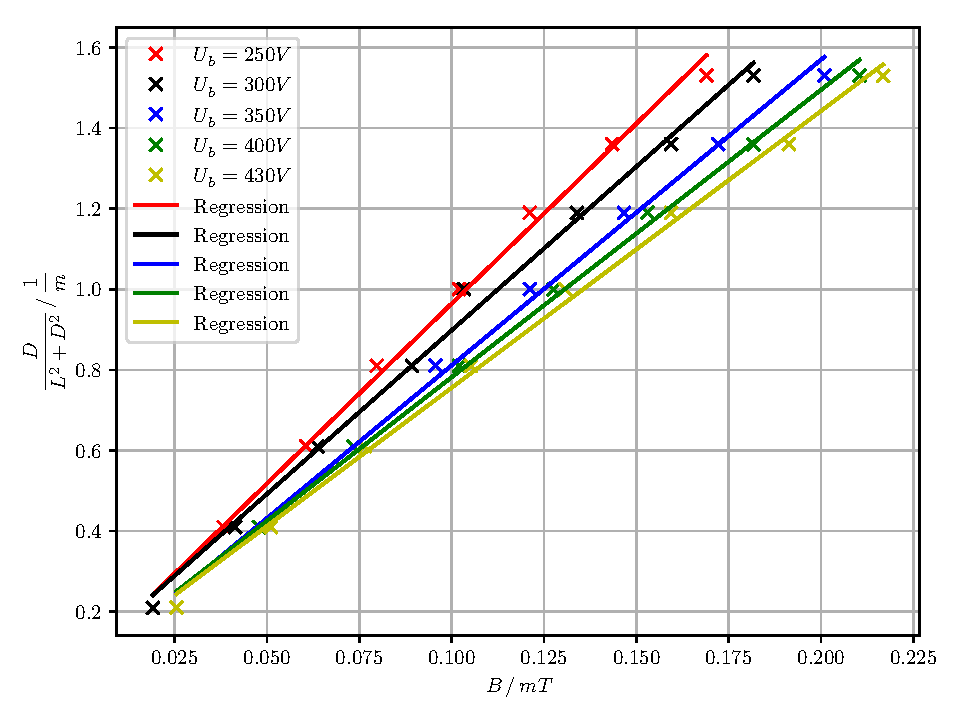
\includegraphics{plot7.pdf}
  \caption{Darstellung von $U_b=\SI{250}{\volt}$.}
  \label{abb:12}
\end{figure}
Die Parameter ergeben sich hierfür
\begin{itemize}
  \item $m = \SI[per-mode=fraction]{8.93(23)}{\per\meter\per\milli\tesla}$
  \item $b =\SI[per-mode=fraction]{0.07(02)}{\per\meter}$
\end{itemize}
Für die nächste wurde eine Beschleunigungsspannung von $U_b = \SI{300}{\volt}$ verwendet.
Sie ist in der Abbildung \ref{abb:13} dargestellt.
\begin{figure}[H]
  \centering
  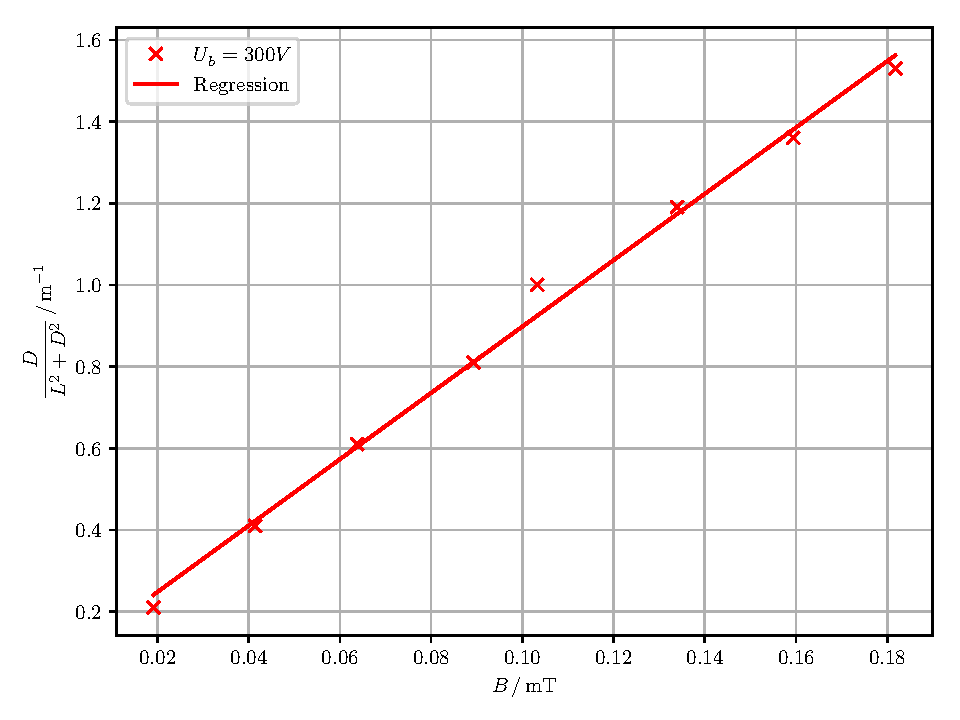
\includegraphics{plot8.pdf}
  \caption{Darstellung von $U_b=\SI{250}{\volt}$.}
  \label{abb:13}
\end{figure}
Die Parameter ergeben sich hierfür
\begin{itemize}
  \item $m = \SI[per-mode=fraction]{8.12(25)}{\per\meter\per\milli\tesla}$
  \item $b =\SI[per-mode=fraction]{0.09(03)}{\per\meter}$
\end{itemize}
Für die nächste wurde eine Beschleunigungsspannung von $U_b = \SI{350}{\volt}$ verwendet.
Sie ist in der Abbildung \ref{abb:14} dargestellt.
\begin{figure}[H]
  \centering
  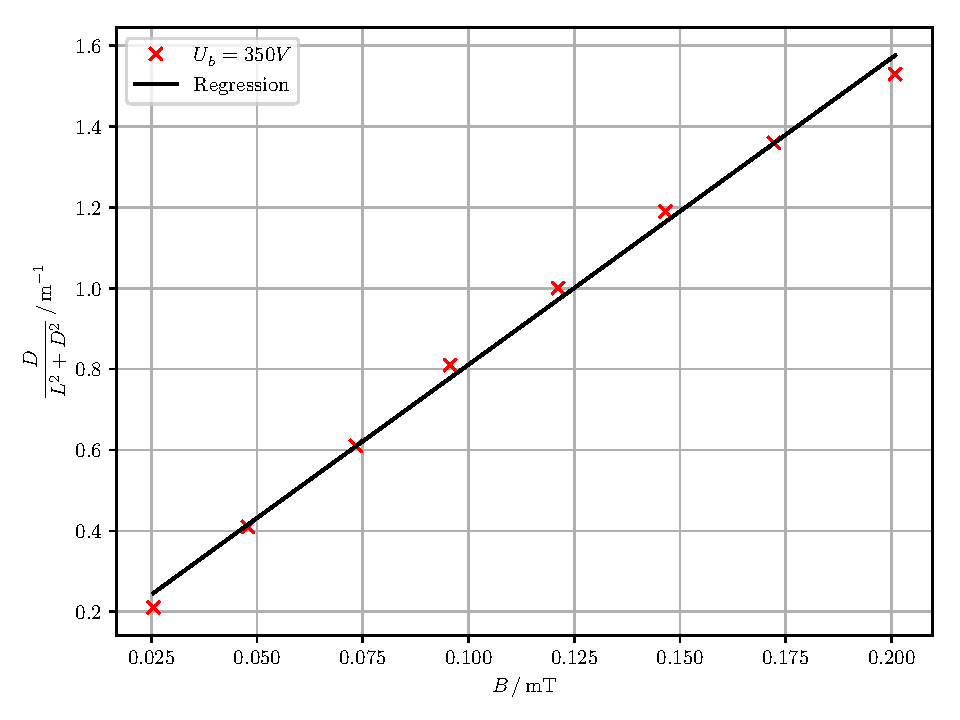
\includegraphics{plot9.pdf}
  \caption{Darstellung von $U_b=\SI{350}{\volt}$.}
  \label{abb:14}
\end{figure}
Die Parameter ergeben sich hierfür
\begin{itemize}
  \item $m = \SI[per-mode=fraction]{7.58(19)}{\per\meter\per\milli\tesla}$
  \item $b =\SI[per-mode=fraction]{0.05(02)}{\per\meter}$
\end{itemize}
Für die nächste wurde eine Beschleunigungsspannung von $U_b = \SI{400}{\volt}$ verwendet.
Sie ist in der Abbildung \ref{abb:15} dargestellt.
\begin{figure}[H]
  \centering
  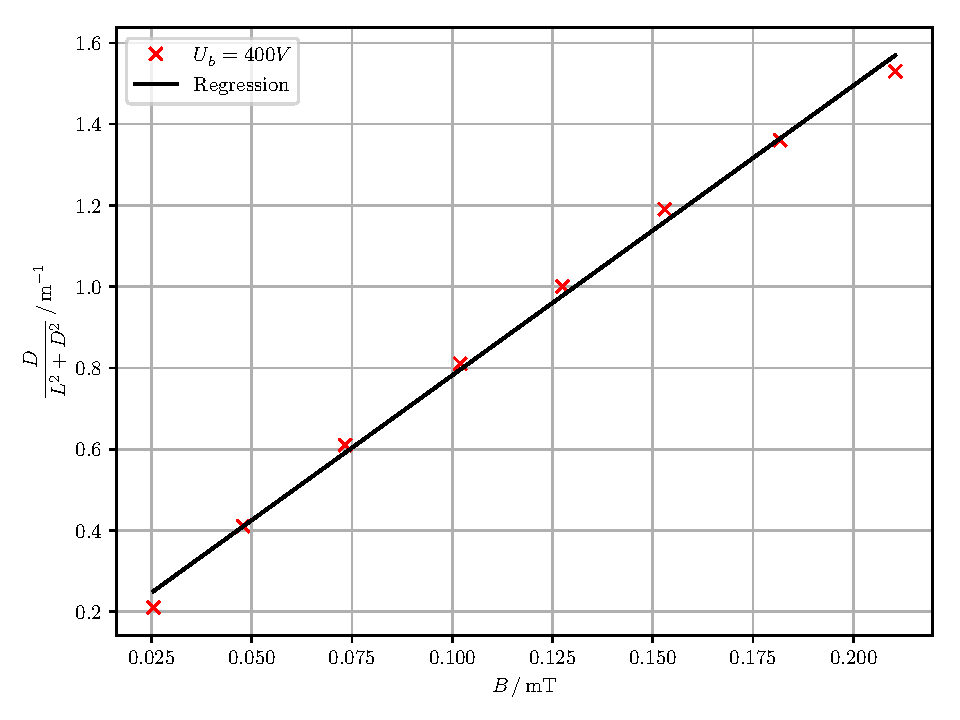
\includegraphics{plot10.pdf}
  \caption{Darstellung von $U_b=\SI{400}{\volt}$.}
  \label{abb:15}
\end{figure}
Die Parameter ergeben sich hierfür
\begin{itemize}
  \item $m = \SI[per-mode=fraction]{7.13(17)}{\per\meter\per\milli\tesla}$
  \item $b =\SI[per-mode=fraction]{0.07(02)}{\per\meter}$
\end{itemize}
Für die nächste wurde eine Beschleunigungsspannung von $U_b = \SI{430}{\volt}$ verwendet.
Sie ist in der Abbildung \ref{abb:16} dargestellt.
\begin{figure}[H]
  \centering
  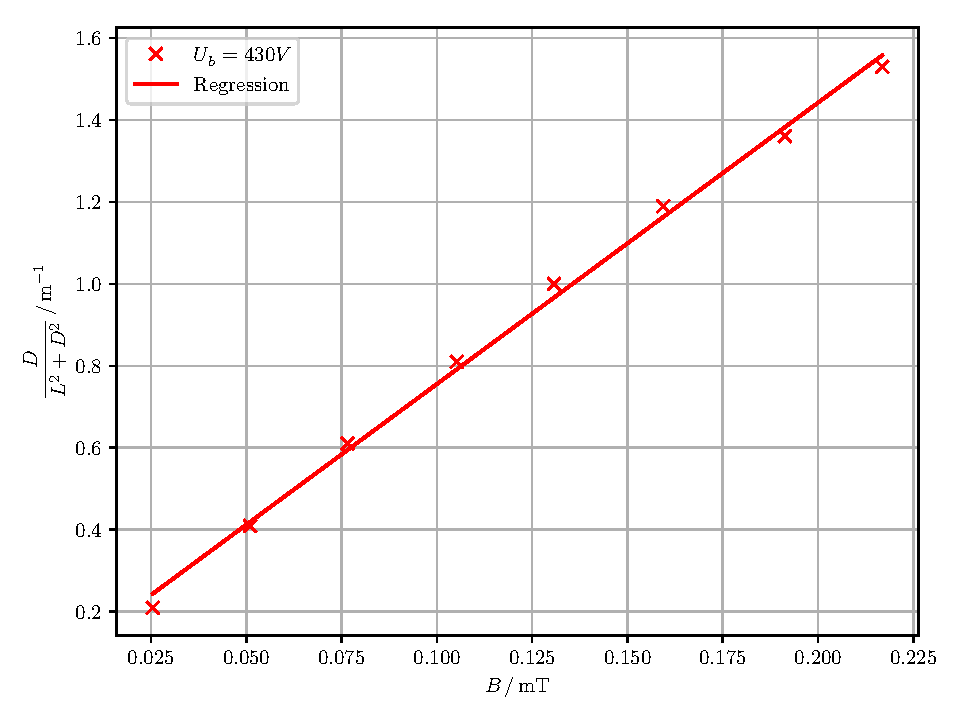
\includegraphics{plot11.pdf}
  \caption{Darstellung von $U_b=\SI{430}{\volt}$.}
  \label{abb:16}
\end{figure}
Die Parameter ergeben sich hierfür
\begin{itemize}
  \item $m = \SI[per-mode=fraction]{6.87(16)}{\per\meter\per\milli\tesla}$
  \item $b =\SI[per-mode=fraction]{0.07(02)}{\per\meter}$
\end{itemize}

Die Ergebnisse für die Bestimmung der spezifische Ladung $\frac{e_0}{m_0}$ werden
in der Tabelle \ref{tab:6} dargestellt. Dabei wurde folgende Rechnung verwendet:
\begin{equation*}
  \frac{e_0}{m_0} = 8 \cdot U_B \cdot m_{i}^2 \,\,\, \text{für} \,\,\, i \in [1,2,3,4,5]
\end{equation*}
Der Fehler lässt sich mit der Gauß´schen Fehlerfortpflanzung bestimmen
\begin{equation*}
  \Delta \frac{e_0}{m_0} = \sqrt{(16 \cdot U_b \cdot m \cdot \Delta m)^2}.
\end{equation*}
Ebenso werden die wichtigen Parameter aus der Messdatenreihe in der Tabelle \ref{tab:6}
dargestellt.

\begin{table}[H]
  \centering
  \caption{Darstellung der spezifische Ladung.}
  \label{tab:6}
  \begin{tabular}{c c c c}
\toprule
$\text{Beschleunigungsspannung}\, U_B \,/\, V$ & $\text{Steigung m} \,/\, \frac{1}{m\cdot mT}$ &$\frac{e_0}{m_0} \,/\, 10^{11}\frac{C}{kg}$ & $\text{Abweichung} \,/\, \%$\\
\midrule
250 &$\num{8.93(23)}$ &$\num{1.59(8)}$ &  9,66\\
300 &$\num{8.12(25)}$ &$\num{1.58(10)}$& 10,23\\
350 &$\num{7.58(19)}$ &$\num{1.61(8)}$ &  8,52\\
400 &$\num{7.13(17)}$ &$\num{1.63(8)}$& 7,39\\
430 &$\num{6.87(16)}$ &$\num{1.62(8)}$& 7,95\\
\bottomrule
  \end{tabular}
\end{table}

Aus den bestimmten spezifischen Ladungen wird nun der Mittelwert und Standardabweichung
bestimmt mit den folgenden Gleichungen.

\begin{equation*}
  \overline{\frac{e_0}{m_0}}= \frac{1}{N} \sum_{i=1}^{N} \frac{e_0}{m_0}_{i}
\end{equation*}
\begin{equation*}
\Delta \overline{\frac{e_0}{m_0}} = \frac{1}{\sqrt{N}\sqrt{N-1}} \sqrt{\sum_{i}\left(\frac{e_0}{m_0}_{i}-\overline{\frac{e_0}{m_0}}\right)^2}
\end{equation*}

Der Mittelwert ergibt sich somit zu:

\begin{equation*}
  \overline{\frac{e_0}{m_0}} = \SI{1.606(92)e11}{\coulomb\per\kilo\gram}
\end{equation*}

Zuletzt soll die Totalintensität des Erdmagnetfeldes errechnet werden.
Aus dem Spulenstrom kann das Magnetfeld, was in der Helmholzspule erzeugt wird,
berechnet werden.
Mit einem gemessenen Spulenstrom von
\begin{equation*}
  I_\text{H} =\SI{126}{\milli\ampere}
\end{equation*}
folgt mit Gleichung \ref{eq:4} für die Magnetfeldstärke:
\begin{equation*}
  B_\text{H} =\SI{8.035}{\micro\tesla}.
\end{equation*}
Zu beachten ist, dass die Magnetfeldstärke $B_\text{H}$ die horizontale Komponente des Erdmagnetfelds ist.
Wichtig hierbei ist in welchem Winkel das Erdmagnetfeld zum Erdboden steht.
Die gemessenen Winkeln sind in der Tabelle \ref{tab:7} dargestellt.
\begin{table}[H]
  \centering
  \caption{Messung des Inklinationwinkels $\varphi$ an verschiedenen Orten.}
  \label{tab:7}
  \begin{tabular}{c}
\toprule
$\text{Winkel}\, \varphi \,/\, \circ$\\
\midrule
82\\
73\\
55\\
55\\
\bottomrule
  \end{tabular}
\end{table}
Mit den folgenden Gleichungen wird der Mittelwert sowie Standardabweichung berechnet.
\begin{equation*}
  \bar{\varphi}= \frac{1}{N} \sum_{i=1}^{N} \varphi_{i}
\end{equation*}
\begin{equation*}
\Delta \bar{\varphi} = \frac{1}{\sqrt{N}\sqrt{N-1}} \sqrt{\sum_{i}(\varphi_{i}-\bar{\varphi})^2}
\end{equation*}
Es folgt somit für den Inklinationswinkel:
\begin{equation*}
  \varphi = \SI{66.25(675)}{\degree}
\end{equation*}
Aus der Überlegung, dass sich das Erdmagnetfeld in zwei Komponente zerlegen lässt, folgt für die Berechnung des Erdmagnetfelds
\begin{equation*}
  B = \frac{B_\text{H}}{\cos(\varphi)}
\end{equation*}
Auch hier lässt sich der Fehler mithilfe der Gauß´schen Fehlerfortpflanzung berechnen
\begin{equation*}
  \Delta B = \sqrt{\Bigl(\frac{B_\text{H} \sin(\varphi)}{\cos^2(\varphi)} \cdot \Delta \varphi\Bigr)^2}
\end{equation*}
Somit ergibt sich für das Erdmagnetfeld:
\begin{equation*}
  B= \SI{20(5)}{\micro\tesla}
\end{equation*}
